\section*{A brief description of the CRISPR circuit using SBOL 2.0 data model}
We first give a brief description of the CRISPR-based repression module. We use bold font in the following text and figure captions to mark available data model in SBOL 2.0.0 Detailed description of properties of the data model is available in the~\href{http://sbolstandard.org/downloads/specification-data-model-2-0/}{Specification
  (Data Model 2.0)}.

First, consider the CRISPR-based Repression Template \sbol{ModuleDefinition} shown in the center of Figure~\ref{fig:fig-CRPb}. It provides a generic description of CRISPR-based repression behavior. Namely, it includes generic \emph{Cas9}, \emph{guide RNA} (gRNA), and \emph{target} DNA \sbol{FunctionalComponent} instances. It also includes a \emph{genetic production} \sbol{Interaction} that expresses a generic target gene product.  Finally, it includes a \emph{non-covalent binding} \sbol{Interaction} that forms the Cas9/gRNA complex (shown as dashed arrows), which in turn participates in an \emph{inhibition} \sbol{Interaction} to repress the target gene product production (shown with a tee-headed arrow). The CRISPR-based Repression Template is then instantiated to test a particular CRISPR-based repression device, CRPb, by the outer CRPb Characterization Circuit \sbol{ModuleDefinition}.  This outer characterization circuit includes gene \sbol{FunctionalComponents} to produce specific products (i.e., mKate, Gal4VP16, cas9m\_BFP, gRNA\_b, and EYFP), as well as \sbol{FunctionalComponents} for the products themselves.  Next, it includes \emph{genetic production} \sbol{Interactions} connecting the genes to their products, and it has a \emph{stimulation} \sbol{Interaction} that indicates that Gal4VP16 stimulates production of EYFP.  Finally, it uses \sbol{MapsTo} objects (shown as dashed lines) to connect the generic \sbol{FunctionalComponents} in the template to the specific objects in the outer \sbol{ModuleDefinition}.  For example, the outer module indicates that the target protein is EYFP, while the cas9\_gRNA complex is cas9m\_BFP\_gRNA\_b.

\begin{figure}[tbph]
\begin{center}
  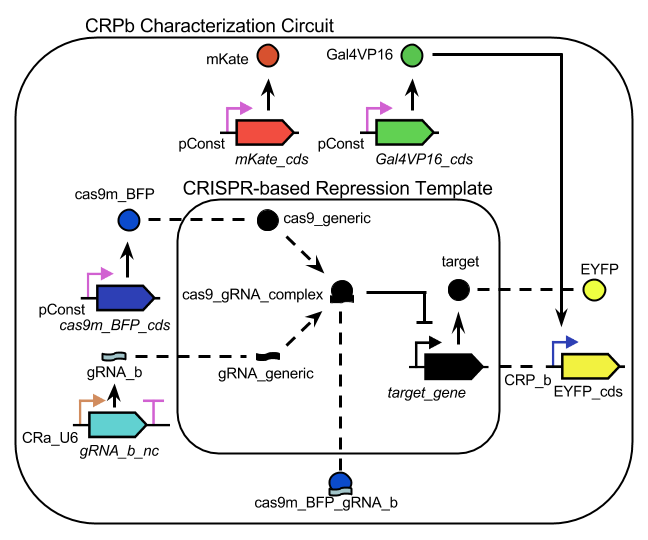
\includegraphics[width=0.95\textwidth]{figures/crispr_repression2} 
\end{center}
\caption{\label{fig:fig-CRPb} Illustration of a hierarchical CRISPR-based repression module represented in SBOL 2.0 (adapted from Figure~1a in \cite{kiani2014crispr}). The CRISPR-based Repression Template \sbol{ModuleDefinition} describes a generic CRISPR repression circuit that combines a Cas9 protein with a gRNA to form a complex (represented by the dashed arrows) that represses a target gene (represented by the arrow with the tee arrowhead).  These relationships between these \sbol{FunctionalComponents} (instances of \sbol{ComponentDefinitions}) are represented in SBOL 2.0 using \sbol{Interactions}.  This \sbol{Module} is instantiated in the outer CRPb Characterization Circuit \sbol{ModuleDefinition} in order to specify the precise (including \sbol{Sequences} when provided) \sbol{FunctionalComponents}  used for each generic \sbol{FunctionalComponent}. The undirected dashed lines going into the template \sbol{Module} represent \sbol{MapsTo} objects that specify how specific \sbol{FunctionalComponents} replace the generic ones.}
\end{figure}

\section*{Modeling CRISPR repression using {\tt libSBOL 2.0.0}}

%\subsection*{Setting up the CRISPR repression model}
%Now we are ready to create the CRISPR model to our project. 
%\begin{center}
% 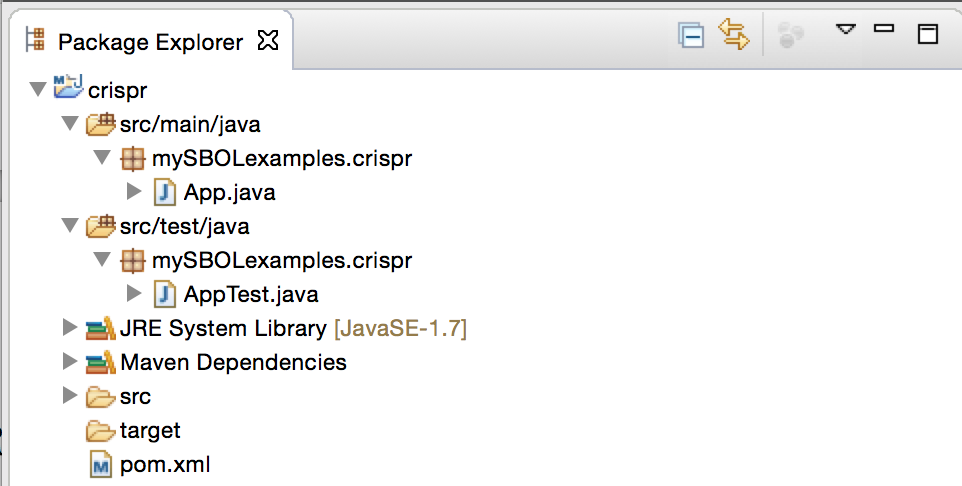
\includegraphics[width=0.8\textwidth]{figures/addCrisprModel1}
%\end{center}


\subsection*{Creating SBOL Document}
 All SBOL data objects are organized within an \sbol{SBOLDocument} object. The \sbol{SBOLDocument} provides a rich set of methods to create, access, update, and delete each type of \sbol{TopLevel} object (i.e., \sbol{Collection}, \sbol{ModuleDefinition}, \sbol{ComponentDefinition}, \sbol{Sequence}, \sbol{Model}, or \sbol{GenericTopLevel}). Every SBOL object has a \emph{uniform resource identifier} (URI) and consists of properties that may refer to other objects, including non-\sbol{TopLevel} objects such as SequenceConstraint and Interaction objects. \texttt{libSBOL 2.0.0} organizes the URI collections to enable efficient access. We first create an \sbol{SBOLDocument} object by calling its constructor as shown below.

\begin{minipage}{0.95\textwidth} 
\begin{lstlisting}
setHomespace("http://sbols.org/CRISPR_Example");
toggleSBOLCompliantTypes();
Document &doc = *new Document();
std::string version = "1.0.0";
\end{lstlisting}
\end{minipage}

The method \lstinline+setHomespace+ sets the
default URI prefix to the string  `http://sbols.org/CRISPR\_Example'. All data objects created following this statement carry this default URI prefix. The author of any SBOL object should use a URI prefix that either they own or an organization of which they are a member owns. Setting a default namespace is like a signature verifying ownership of objects. 

\subsection*{Adding CRISPR-based Repression Template module}
\subsubsection*{Creating \sbol{TopLevel} objects}
We first create the CRISPR-based Repression Template module shown in
Figure~\ref{fig:fig-CRPb}. In this template, we include definitions
for generic \emph{Cas9}, \emph{guide RNA} (gRNA), and \emph{target}
DNA \sbol{FunctionalComponent} instances. They are encoded as
\sbol{ComponentDefinition} objects. With \sbol{FunctionalComponent}, optional fields such as \emph{direction} are used to specify the input, output, both, or neither with regards to the \sbol{ModuleDefinition} that contains it. Creation of the generic Cas9 (line
2) \sbol{ComponentDefinition} is done by passing its \emph{displayId}
``cas9\_generic''.  The displayId is appended to the default namespace to create the URI "http://sbols.org/CRISPR\_Example/cas9\_generic.  The next argument is the required field, 
\emph{type}. Every \sbol{ComponentDefinition} must contain one or more
types, each of which is specified by a URI. A type specifies the
component's category of biochemical or physical entity (for example
DNA, protein, or small molecule). The generic Cas9's type is
\lstinline+BIOPAX_PROTEIN+(\url{http://www.biopax.org/release/biopax-level3.owl\#Protein}), which is defined as the BioPAX ontology term for
protein.  Finally, an optional \emph{version} specified by the \lstinline+version+
string may be specied. If \emph{version} is not specified, it will be set by default to 1.0.0
. Other
\sbol{ComponentDefinition} objects shown below are created in the same
way. A \sbol{ComponentDefinition} object can optionally have one or
more roles, also in the form of URIs. The \lstinline+gRNA_generic+ has
a role of \lstinline+SGRNA+ (line 7 below), defined as the
\emph{Sequence Ontology} (SO) term ``SO:0001998''.
(\url{http://identifiers.org/so/SO:0001998}) in the
library. Similarly, the \lstinline+target_gene+ on line 16 below has a role of
\lstinline+PROMOTER+, defined as SO term ``SO:0000167''
(\url{http://identifiers.org/so/SO:0000167}). We then create the \sbol{ModuleDefinition} template by constructing a \lstinline+ModuleDefinition+ with the displayId ``CRISPR\_Template''.

\vspace{\abovedisplayskip}
\begin{minipage}{0.95\textwidth} 
\begin{lstlisting}
// Create ComponentDefinition for cas9_generic protein
ComponentDefinition& cas9_generic = *new ComponentDefinition("cas9_generic", BIOPAX_PROTEIN, version);
doc.add<ComponentDefinition>(cas9_generic);

// Create ComponentDefinition for gRNA_generic RNA
ComponentDefinition& gRNA_generic = *new ComponentDefinition("gRNA_generic", BIOPAX_RNA, version);
gRNA_generic.roles.set("http://identifiers.org/so/SO:0001998");
doc.add<ComponentDefinition>(gRNA_generic);

// Create ComponentDefinition for cas9_gRNA_complex
ComponentDefinition& cas9_gRNA_complex = *new ComponentDefinition("cas9_gRNA_complex", BIOPAX_COMPLEX, version);
doc.add<ComponentDefinition>(cas9_gRNA_complex);

// Create ComponentDefinition for target gene
ComponentDefinition& target_gene = *new ComponentDefinition("target_gene", BIOPAX_DNA, version);
target_gene.roles.set(SO_PROMOTER);
doc.add<ComponentDefinition>(target_gene);

// Create ComponentDefinition for target protein
ComponentDefinition& target = *new ComponentDefinition("target", BIOPAX_PROTEIN, version);
doc.add<ComponentDefinition>(target);

// Create ModuleDefinition for CRISPR_Repression_Template	
ModuleDefinition &CRISPR_Template = *new ModuleDefinition("CRISPR_Template", version);
doc.add<ModuleDefinition>(CRISPR_Template);
\end{lstlisting}
\end{minipage}

By default, libSBOL operates in SBOL-compliant mode. In SBOL-compliant mode, each constructor creates an SBOL-compliant URI with the following form:
\begin{center}
http://$\langle$prefix$\rangle$/$\langle$displayId$\rangle$/$\langle$version$\rangle$
\end{center}
using the default URI prefix and provided displayId and version. The \emph{$\langle$prefix$\rangle$} represents a URI for a namespace (for example, {\tt www.sbols.org/CRISPR\_Example}).  When using compliant URIs, the owner of a prefix must ensure that the URI of any unique \sbol{TopLevel} object that contains the prefix also contains a unique  \emph{$\langle$displayId$\rangle$} or \emph{$\langle$version$\rangle$} portion. Multiple versions of an SBOL object can exist and would have compliant URIs that contain identical prefixes and displayIds, but each of these URIs would need to end with a unique version. Lastly, the compliant URI of a non-\sbol{TopLevel} object is identical to that of its parent object, except that its displayId is inserted between its parent's displayId and version. This form of compliant URIs is chosen to be easy to read, facilitate debugging, and support a more efficient means of looking up objects and checking URI uniqueness.

\subsubsection*{Specifying Interactions}
We are now ready to specify the interactions in the repression template. The first one is the complex formation interaction for \lstinline+cas9_generic+ and \lstinline+gRNA_generic+. We first create an \sbol{Interaction} object \lstinline+cas9_complex_formation+ in \lstinline+CRISPR_Template+, with the displayId ``cas9\_complex\_formation'' and a non-covalent binding type (line 1 to 2). It is recommended that terms from the \emph{Systems Biology Ontology} (SBO)~\cite{Courtot2011} are used specify the types for interactions. Table 11 of the ~\href{http://sbolstandard.org/downloads/specification-data-model-2-0/}{Specification  (Data Model 2.0)} document provides a list of possible SBO terms for the types property and their corresponding URIs. 

Next, we create three participants to this interaction object. Each participant represents a species participating in a biochemical reaction. The components which participate in an interaction must be assigned using the \lstinline+participate+method.

\vspace{\abovedisplayskip}
\begin{minipage}{0.95\textwidth}%{\linewidth} 
\begin{lstlisting}
Interaction &Cas9Complex_Formation = CRISPR_Template.interactions.create("cas9_complex_formation");
Cas9Complex_Formation.types.set(SBO_NONCOVALENT_BINDING);

FunctionalComponent &cas9_generic_fc = CRISPR_Template.functionalComponents.create("cas9_generic");
cas9_generic_fc.definition.set(cas9_generic.persistentIdentity.get());
cas9_generic_fc.access.set(SBOL_ACCESS_PUBLIC);
cas9_generic_fc.direction.set(SBOL_DIRECTION_IN_OUT);
cas9_generic_fc.version.set(version);

Participation &cas9_generic_participation = Cas9Complex_Formation.participations.create("cas9_generic");
cas9_generic_participation.roles.set(SBO_REACTANT);
cas9_generic_participation.participant.set(cas9_generic_fc.identity.get());

FunctionalComponent &gRNA_generic_fc = CRISPR_Template.functionalComponents.create("gRNA_generic");
gRNA_generic_fc.definition.set(gRNA_generic.persistentIdentity.get());
gRNA_generic_fc.access.set(SBOL_ACCESS_PUBLIC);
gRNA_generic_fc.direction.set(SBOL_DIRECTION_IN_OUT);
gRNA_generic_fc.version.set(version);

Participation &gRNA_generic_participation = Cas9Complex_Formation.participations.create("gRNA_generic"); 
gRNA_generic_participation.roles.set(SBO_REACTANT);
gRNA_generic_participation.participant.set(gRNA_generic_fc.identity.get());

FunctionalComponent &cas9_gRNA_complex_fc = CRISPR_Template.functionalComponents.create("cas9_gRNA_complex");
cas9_gRNA_complex_fc.definition.set(cas9_gRNA_complex.persistentIdentity.get());
cas9_gRNA_complex_fc.access.set(SBOL_ACCESS_PUBLIC);
cas9_gRNA_complex_fc.direction.set(SBOL_DIRECTION_IN_OUT);
cas9_gRNA_complex_fc.version.set(version);

Participation &cas9_gRNA_complex_participation = Cas9Complex_Formation.participations.create("cas9_gRNA_complex");
cas9_gRNA_complex_participation.roles.set(SBO_PRODUCT);
cas9_gRNA_complex_participation.participant.set(cas9_gRNA_complex_fc.identity.get());
\end{lstlisting}
\end{minipage}

The remaining two interactions, namely the genetic production of the target protein from the \lstinline+target_gene+ and the inhibition of the target protein by the \lstinline+cas9_gRNA_complex+, are specified using the same method calls.

\vspace{\abovedisplayskip}
\begin{minipage}{0.95\textwidth}%{\linewidth} 
\begin{lstlisting}
// Production of target from target gene
Interaction &EYFP_production = CRISPR_Template.interactions.create("target_production"); 
EYFP_production.types.set(SBO_GENETIC_PRODUCTION);

FunctionalComponent &target_gene_fc = CRISPR_Template.functionalComponents.create("target_gene");
target_gene_fc.definition.set(target_gene.persistentIdentity.get());
target_gene_fc.access.set(SBOL_ACCESS_PUBLIC);
target_gene_fc.direction.set(SBOL_DIRECTION_IN_OUT);
target_gene_fc.version.set(version);

Participation &target_gene_participation = EYFP_production.participations.create("target_gene"); 
target_gene_participation.roles.set(SBO_PROMOTER);
target_gene_participation.participant.set(target_gene_fc.identity.get());

FunctionalComponent &target_fc = CRISPR_Template.functionalComponents.create("target");
target_fc.definition.set(target.persistentIdentity.get());
target_fc.access.set(SBOL_ACCESS_PUBLIC);
target_fc.direction.set(SBOL_DIRECTION_IN_OUT);
target_fc.version.set(version);

Participation &target_participation = EYFP_production.participations.create("target"); 
target_participation.roles.set(SBO_PRODUCT);
target_participation.participant.set(target_fc.identity.get());

// Inhibition of target by cas9m_BFP_gRNA 
Interaction &target_generic_gene_inhibition = CRISPR_Template.interactions.create("target_gene_inhibition"); 
target_generic_gene_inhibition.types.set(SBO_INHIBITION);

Participation &cas9_gRNA_complex_participation1 = target_generic_gene_inhibition.participations.create("cas9_gRNA_complex");
cas9_gRNA_complex_participation1.roles.set(SBO_INHIBITOR);
cas9_gRNA_complex_participation1.participant.set(cas9_gRNA_complex_fc.identity.get());
	
Participation &target_gene_participation2 = target_generic_gene_inhibition.participations.create("target_gene"); 
target_gene_participation2.roles.set(SBO_PROMOTER);
target_gene_participation2.participant.set(target_gene_fc.identity.get());
\end{lstlisting}
\end{minipage}

\subsection*{Creating CRPb Characterization Circuit}
So far, we have completed the repression template. In order to construct the the CRPb Characterization Circuit, we must realize the template with specific components. We first create \sbol{Sequence} objects for those provided in \cite{kiani2014crispr}\footnote{Unfortunately, as usual, not all sequences are provided in the paper.} as shown in the code below. For example, to create the sequence for the CRP\_b promoter, we call the \lstinline+Sequence+constructor, as shown on line 53, with the displayId ``CRP\_b\_seq'', \lstinline+version+, the sequence specified by \lstinline+CRP_b_seq_elements+, and the IUPAC encoding for DNA, which is defined as a URI in the \sbol{Sequence} class, referencing \url{http://www.chem.qmul.ac.uk/iubmb/misc/naseq.html}.

\vspace{\abovedisplayskip}
\begin{minipage}{0.95\textwidth}%{\linewidth} 
\begin{lstlisting}[basicstyle=\tt\footnotesize]
// Create Sequence for CRa_U6 promoter
std::string CRa_U6_seq_elements ="GGTTTACCGAGCTCTTATTGGTTTTCAAACTTCATTGACTGTGCC" 
										"AAGGTCGGGCAGGAAGAGGGCCTATTTCCCATGATTCCTTCATAT" 
										"TTGCATATACGATACAAGGCTGTTAGAGAGATAATTAGAATTAAT" 
										"TTGACTGTAAACACAAAGATATTAGTACAAAATACGTGACGTAGA" 
										"AAGTAATAATTTCTTGGGTAGTTTGCAGTTTTAAAATTATGTTTT" 
										"AAAATGGACTATCATATGCTTACCGTAACTTGAAATATAGAACCG" 
										"ATCCTCCCATTGGTATATATTATAGAACCGATCCTCCCATTGGCT" 
										"TGTGGAAAGGACGAAACACCGTACCTCATCAGGAACATGTGTTTA" 
										"AGAGCTATGCTGGAAACAGCAGAAATAGCAAGTTTAAATAAGGCT" 
										"AGTCCGTTATCAACTTGAAAAAGTGGCACCGAGTCGGTGCTTTTT" 
										"TTGGTGCGTTTTTATGCTTGTAGTATTGTATAATGTTTTT";
Sequence& CRa_U6_seq = *new Sequence("CRa_U6_seq", CRa_U6_seq_elements, SBOL_ENCODING_IUPAC, version);
doc.add<Sequence>(CRa_U6_seq);

// Create Sequence for gRNA_b coding sequence
std::string gRNA_b_elements = "AAGGTCGGGCAGGAAGAGGGCCTATTTCCCATGATTCCTTCATAT" 
		"TTGCATATACGATACAAGGCTGTTAGAGAGATAATTAGAATTAAT" 
		"TTGACTGTAAACACAAAGATATTAGTACAAAATACGTGACGTAGA" 
		"AAGTAATAATTTCTTGGGTAGTTTGCAGTTTTAAAATTATGTTTT" 
		"AAAATGGACTATCATATGCTTACCGTAACTTGAAAGTATTTCGAT" 
		"TTCTTGGCTTTATATATCTTGTGGAAAGGACGAAACACCGTACCT" 
		"CATCAGGAACATGTGTTTAAGAGCTATGCTGGAAACAGCAGAAAT" 
		"AGCAAGTTTAAATAAGGCTAGTCCGTTATCAACTTGAAAAAGTGG" 
		"CACCGAGTCGGTGCTTTTTTT";
Sequence& gRNA_b_seq = *new Sequence("gRNA_b_seq", gRNA_b_elements, SBOL_ENCODING_IUPAC, version);
doc.add<Sequence>(gRNA_b_seq);

// Create Sequence for mKate
std::string mKate_seq_elements = "TCTAAGGGCGAAGAGCTGATTAAGGAGAACATGCACATGAAGCTG" 
		"TACATGGAGGGCACCGTGAACAACCACCACTTCAAGTGCACATCC" 
		"GAGGGCGAAGGCAAGCCCTACGAGGGCACCCAGACCATGAGAATC" 
		"AAGGTGGTCGAGGGCGGCCCTCTCCCCTTCGCCTTCGACATCCTG" 
		"GCTACCAGCTTCATGTACGGCAGCAAAACCTTCATCAACCACACC" 
		"CAGGGCATCCCCGACTTCTTTAAGCAGTCCTTCCCTGAGGTAAGT" 
		"GGTCCTACCTCATCAGGAACATGTGTTTTAGAGCTAGAAATAGCA" 
		"AGTTAAAATAAGGCTAGTCCGTTATCAACTTGAAAAAGTGGCACC" 
		"GAGTCGGTGCTACTAACTCTCGAGTCTTCTTTTTTTTTTTCACAG" 
		"GGCTTCACATGGGAGAGAGTCACCACATACGAAGACGGGGGCGTG" 
		"CTGACCGCTACCCAGGACACCAGCCTCCAGGACGGCTGCCTCATC" 
		"TACAACGTCAAGATCAGAGGGGTGAACTTCCCATCCAACGGCCCT" 
		"GTGATGCAGAAGAAAACACTCGGCTGGGAGGCCTCCACCGAGATG" 
		"CTGTACCCCGCTGACGGCGGCCTGGAAGGCAGAAGCGACATGGCC" 
		"CTGAAGCTCGTGGGCGGGGGCCACCTGATCTGCAACTTGAAGACC" 
		"ACATACAGATCCAAGAAACCCGCTAAGAACCTCAAGATGCCCGGC" 
		"GTCTACTATGTGGACAGAAGACTGGAAAGAATCAAGGAGGCCGAC" 
		"AAAGAGACCTACGTCGAGCAGCACGAGGTGGCTGTGGCCAGATAC" 
		"TGCG";
Sequence& mKate_seq = *new Sequence("mKate_seq", mKate_seq_elements, SBOL_ENCODING_IUPAC, version);
doc.add<Sequence>(mKate_seq);

// Create Sequence for CRP_b promoter
std::string CRP_b_seq_elements = "GCTCCGAATTTCTCGACAGATCTCATGTGATTACGCCAAGCTACG" 
		"GGCGGAGTACTGTCCTCCGAGCGGAGTACTGTCCTCCGAGCGGAG" 
		"TACTGTCCTCCGAGCGGAGTACTGTCCTCCGAGCGGAGTTCTGTC" 
		"CTCCGAGCGGAGACTCTAGATACCTCATCAGGAACATGTTGGAAT" 
		"TCTAGGCGTGTACGGTGGGAGGCCTATATAAGCAGAGCTCGTTTA" 
		"GTGAACCGTCAGATCGCCTCGAGTACCTCATCAGGAACATGTTGG" 
		"ATCCAATTCGACC"; 
Sequence& CRP_b_seq = *new Sequence("CRP_b_seq", CRP_b_seq_elements, SBOL_ENCODING_IUPAC, version);
doc.add<Sequence>(CRP_b_seq);
\end{lstlisting}
\end{minipage}

Next, we specify \sbol{ComponentDefinitions} for all \sbol{FunctionalComponents} in the CRPb Characterization Circuit. The code snippet below first creates a \sbol{ComponentDefinition} of DNA type for the \lstinline+CRP_b+ promoter (lines 2-5). Then, we create two \sbol{ComponentDefinition} objects, one for the EYFP \emph{coding sequence} (CDS) and another for the EYFP gene (lines 8-15). We use a \sbol{SequenceConstraint} object (lines 27-30) to indicate that the \lstinline+CRP_b+ promoter precedes the \lstinline+EYFP_cds+, because the sequence for the CDS has not been provided and thus cannot be given an exact \sbol{Range}. The \sbol{restriction} property uses flags defined in the formal specification, which are provided in libSBOL as predefined constants.  See the API documentation or the constants.h header file for predefined constants associated with an SBOL property.

\vspace{\abovedisplayskip}
\begin{minipage}{0.95\textwidth}
\begin{lstlisting}
// Create ComponentDefinition for CRP_b promoter
ComponentDefinition& CRP_b = *new ComponentDefinition("CRP_b", BIOPAX_DNA, version);
CRP_b.roles.set(SO_PROMOTER);
CRP_b.sequences.add(CRP_b_seq.persistentIdentity.get());
doc.add<ComponentDefinition>(CRP_b);

// Create ComponentDefintiion for EYFP coding sequence
ComponentDefinition& EYFP_cds = *new ComponentDefinition("EYFP_cds", BIOPAX_DNA, version);
EYFP_cds.roles.set(SO_CDS);
doc.add<ComponentDefinition>(EYFP_cds);

// Create ComponentDefinition for EYFP gene
ComponentDefinition& EYFP_gene = *new ComponentDefinition("EYFP_gene", BIOPAX_DNA, version);
EYFP_gene.roles.set(SO_PROMOTER);
doc.add<ComponentDefinition>(EYFP_gene);

Component &CRP_b_c = EYFP_gene.components.create("CRP_b");
CRP_b_c.definition.set(CRP_b.persistentIdentity.get());
CRP_b_c.access.set(SBOL_ACCESS_PUBLIC);
CRP_b_c.version.set(version);

Component &EYFP_cds_c = EYFP_gene.components.create("EYFP_cds");
EYFP_cds_c.definition.set(EYFP_cds.persistentIdentity.get());
EYFP_cds_c.access.set(SBOL_ACCESS_PUBLIC);
EYFP_cds_c.version.set(version);

SequenceConstraint &EYFP_gene_constraint = EYFP_gene.sequenceConstraints.create("EYFP_gene_constraint");
EYFP_gene_constraint.subject.set(CRP_b_c.identity.get());
EYFP_gene_constraint.object.set(EYFP_cds_c.identity.get());
EYFP_gene_constraint.restriction.set(SBOL_RESTRICTION_PRECEDES)
\end{lstlisting}
\end{minipage}

Other \sbol{ComponentDefinition} objects can be created using the same set of method calls. As an exercise, the reader is encouraged to specify them according to Table~\ref{tbl:tbl-ComponentDef} and~\ref{tbl:tbl-SeqConstraint}. Entries ``type'' and ``roles'' column in the table are libSBOL constants corresponding to a SequenceOntology term. URIs for these terms are described in Table 3 of the~\href{http://sbolstandard.org/downloads/specification-data-model-2-0/}{Specification  (Data Model 2.0)} document.

\begin{table}[tb]
\centering
\caption{\sbol{ComponentDefinition} objects}
\label{tbl:tbl-ComponentDef}
\begin{tabular}
{c@{\hspace{1.5em}}c@{\hspace{1.5em}}cc@{\hspace{1.5em}}c}
\hline
component definition&
type&
role&
sequence&
sequence constraint\\
\hline
pConst&BIOPAX\_DNA&SO\_PROMOTER&n/a&n/a\\ %
cas9m\_BFP\_cds&BIOPAX\_DNA&SO\_CDS&n/a&n/a\\ %
cas9m\_BFP\_gene&BIOPAX\_DNA&SO\_PROMOTER&n/a&cas9m\_BFP\_gene\_constraint\\%
cas9m\_BFP&BIOPAX\_PROTEIN&n/a&n/a&n/a\\%
CRa\_U6&BIOPAX\_DNA&SO\_PROMOTER&CRa\_U6\_seq&n/a\\%
gRNA\_b\_nc&BIOPAX\_DNA&SO\_CDS&gRNA\_b\_seq&n/a\\%
gRNA\_b\_terminator&BIOPAX\_DNA&SO\_TERMINATOR&n/a&n/a\\%
gRNA\_b\_gene&BIOPAX\_DNA&SO\_PROMOTER&n/a&\begin{tabular}{@{}c@{}}\shortstack{\small{gRNA\_b\_gene\_constraint1} \\ \small{gRNA\_b\_gene\_constraint2}}\end{tabular}\\%
gRNA\_b&BIOPAX\_RNA&SGRNA&n/a&n/a\\%
cas9m\_BFP\_gRNA\_b&BIOPAX\_COMPLEX&n/a&n/a&n/a\\%
mKate\_cds&BIOPAX\_DNA&SO\_CDS&mKate\_seq&n/a\\%
mKate\_gene&BIOPAX\_DNA&SO\_PROMOTER&n/a&mKate\_gene\_constraint\\%
mKate&BIOPAX\_PROTEIN&n/a&n/a&n/a\\%
Gal4VP16\_cds&BIOPAX\_DNA&SO\_CDS&n/a&n/a\\%
Gal4VP16\_gene&BIOPAX\_DNA&SO\_PROMOTER&n/a&GAL4VP16\_gene\_constraint\\%
Gal4VP16&BIOPAX\_PROTEIN&n/a&n/a&n/a\\%
CRP\_b&BIOPAX\_DNA&SO\_PROMOTER&CRP\_b\_seq&n/a\\%
EYFP\_cds&BIOPAX\_DNA&SO\_CDS&n/a&n/a\\%
EYFP\_gene&BIOPAX\_DNA&SO\_PROMOTER&n/a&EYFP\_gene\_constraint\\%
EYFP&BIOPAX\_PROTEIN&n/a&n/a&n/a\\%
\hline
\end{tabular}%

\centering
\caption{\sbol{SequenceConstraint} objects}
\label{tbl:tbl-SeqConstraint}
\begin{tabular}{c@{\hspace{1.5em}}c@{\hspace{1.5em}}cc@{\hspace{1.5em}}c}
\hline
displayId&
restriction type&
subject&
object\\
\hline
cas9m\_BFP\_gene\_constraint&SBOL\_RESTRICTION\_PRECEDES&pConst&cas9m\_BFP\_cds\\%
gRNA\_b\_gene\_constraint1&SBOL\_RESTRICTION\_PRECEDES&CRa\_U6&gRNA\_b\_nc\\%
gRNA\_b\_gene\_constraint2&SBOL\_RESTRICTION\_PRECEDES&gRNA\_b\_nc&gRNA\_b\_terminator\\%
mKate\_gene\_constraint&SBOL\_RESTRICTION\_PRECEDES&pConst&mKate\_cds\\%
GAL4VP16\_gene\_constraint&SBOL\_RESTRICTION\_PRECEDES&pConst&Gal4VP16\_cds\\%
EYFP\_gene\_constraint&SBOL\_RESTRICTION\_PRECEDES&CRP\_b&EYFP\_cds\\%
\end{tabular}
\end{table}

We are now ready to create the CRPb Characterization Circuit which realizes the template design.  We first create a \sbol{ModuleDefinition} object as shown below: 

\vspace{\abovedisplayskip}
\begin{minipage}{0.95\textwidth}
\begin{lstlisting}
// Create ModuleDefintion for CRISPR Repression
ModuleDefinition &CRPb_circuit = *new ModuleDefinition("CRPb_characterization_Circuit", version);
doc.add<ModuleDefinition>(CRPb_circuit);
\end{lstlisting}
\end{minipage}

Next, we need to specify all interactions for the CRPb Characterization Circuit. Following the same procedure for creating \sbol{Interactions} before, we can create those specified in Table~\ref{tbl:tbl-Interaction}. 

\begin{table}[tb]
\caption{\sbol{Interaction} objects}
\label{tbl:tbl-Interaction}
\centering
{\small
\begin{tabular}{c@{\hspace{1.5em}}c@{\hspace{1.5em}}c@{\hspace{1.5em}}c@{\hspace{1.5em}}}
\hline
interaction&
type&
participant&
role\\
\hline
\multirow{2}{*}{mKate\_production}&\multirow{2}{*}{SBO\_GENETIC\_PRODUCTION}&mKate\_gene&SBO\_PROMOTER\\
  &&mKate&SBO\_PRODUCT\\ \hline %
\multirow{2}{*}{Gal4VP16\_production}&\multirow{2}{*}{SBO\_GENETIC\_PRODUCTION}&Gal4VP16\_gene&SBO\_PROMOTER\\
  &&Gal4VP16&PRODUCT\\ \hline %
\multirow{2}{*}{cas9m\_BFP\_production}&\multirow{2}{*}{SBO\_GENETIC\_PRODUCTION}&cas9m\_BFP\_gene&SBO\_PROMOTER\\
  &&cas9m\_BFP&PRODUCT\\ \hline %
\multirow{2}{*}{gRNA\_b\_production}&\multirow{2}{*}{SBO\_GENETIC\_PRODUCTION}&gRNA\_b\_gene&SBO\_PROMOTER\\
  &&gRNA\_b&SBO\_PRODUCT\\ \hline %
\multirow{2}{*}{EYFP\_Activation}&\multirow{2}{*}{SBO\_STIMULATION}&EYFP\_gene&SBO\_PROMOTER\\
  &&Gal4VP16&SBO\_STIMULATOR\\ \hline %
mKate\_deg&SBO\_DEGRADATION&mKate&SBO\_REACTANT\\ \hline%
Gal4VP16\_deg&SBO\_DEGRADATION&Gal4VP16&SBO\_REACTANT\\ \hline%
cas9m\_BFP\_deg&SBO\_DEGRADATION&cas9m\_BFP&SBO\_REACTANT\\ \hline%
gRNA\_b\_deg&SBO\_DEGRADATION&gRNA\_b&SBO\_REACTANT\\ \hline%
EYFP\_deg&SBO\_DEGRADATION&EYFP&SBO\_REACTANT\\ \hline%
cas9m\_BFP\_gRNA\_b\_deg&SBO\_DEGRADATION&cas9m\_BFP\_gRNA\_b&SBO\_REACTANT\\ \hline%
\end{tabular}
}
\end{table}

Now, the CRISPR-based Repression Template can be connected to the CRPb Characterization Circuit using \sbol{Modules}. \sbol{Modules} are used to instantiates a submodule in the parent \sbol{ModuleDefinition}. \sbol{MapsTo} is then created to provide an identity relationship between two \sbol{ComponentInstance} objects, the first contained by the “lower level” definition of the \sbol{ComponentInstance} or \sbol{Module} that owns the MapsTo, and the second contained by the
“higher level” definition that contains the \sbol{ComponentInstance} or \sbol{Module} that owns the \sbol{MapsTo}. The remote property of a \sbol{MapsTo} refers to the first “lower level” \sbol{ComponentInstance}, while the local property refers to the second “higher level” \sbol{ComponentInstance}. 



% This method instantiates a submodule in the parent ModuleDefinition. Note that the argument to this method is an std::vector of ModuleDefinitions, in case one wants to add multiple submodules to a parent \sbol{ModuleDefinition}. Next we use the \lstinline+mask+ method to indicate that the \texttt{target\_gene} in the template should be refined to be the \texttt{EYFP\_gene} specified in the CRPb circuit. This method auto-constructs \sbol{MapsTo} objects with the correct \sbol{refinement} field.

% Code inserted to generate MapsTo but does not compile for 
% CRPb_circuit.assemble({ CRISPR_template });
% EYFP_cds.mask(target_gene);
% cas9_mBFP.mask(cas9_generic);
% gRNA_b.mask(gRNA_generic);

\vspace{\abovedisplayskip}
\begin{minipage}{0.95\textwidth}
\begin{lstlisting}
Module &CRISPR_Template_Module = CRPb_circuit.modules.create("CRISPR_Template"); 	
CRISPR_Template_Module.definition.set(CRISPR_Template.identity.get());

MapsTo &cas9m_BFP_map = CRISPR_Template_Module.mapsTos.create("cas9m_BFP_map");
cas9m_BFP_map.refinement.set(SBOL_REFINEMENT_USE_LOCAL);
cas9m_BFP_map.local.set(cas9m_BFP_fc.identity.get());
cas9m_BFP_map.remote.set(cas9_generic_fc.identity.get());

MapsTo &gRNA_b_map = CRISPR_Template_Module.mapsTos.create("gRNA_b_map");
gRNA_b_map.refinement.set(SBOL_REFINEMENT_USE_LOCAL);
gRNA_b_map.local.set(gRNA_b_fc.identity.get());
gRNA_b_map.remote.set(gRNA_generic_fc.identity.get());

MapsTo &cas9m_BFP_gRNA_map = CRISPR_Template_Module.mapsTos.create("cas9m_BFP_gRNA_map");
cas9m_BFP_gRNA_map.refinement.set(SBOL_REFINEMENT_USE_LOCAL);
cas9m_BFP_gRNA_map.local.set(cas9m_BFP_gRNA_fc.identity.get());
cas9m_BFP_gRNA_map.remote.set(cas9_gRNA_complex_fc.identity.get());

MapsTo &EYFP_map = CRISPR_Template_Module.mapsTos.create("EYFP_map");
EYFP_map.refinement.set(SBOL_REFINEMENT_USE_LOCAL);
EYFP_map.local.set(EYFP_fc.identity.get());
EYFP_map.remote.set(target_fc.identity.get());

MapsTo &EYFP_gene_map = CRISPR_Template_Module.mapsTos.create("EYFP_gene_map");
EYFP_gene_map.refinement.set(SBOL_REFINEMENT_USE_LOCAL);
EYFP_gene_map.local.set(EYFP_gene_fc.identity.get());
EYFP_gene_map.remote.set(target_gene_fc.identity.get());
\end{lstlisting}
\end{minipage}

At this point, we have completed the CRISPR circuit model. 

One final step is to serialize the complete model to produce an RDF/XML output. This can be done by adding the code below.

\vspace{\abovedisplayskip}
\begin{minipage}{0.95\textwidth}
\begin{lstlisting}
doc.write("CRISPR_example.xml");
\end{lstlisting}
\end{minipage}